
Biểu đồ Gantt kế hoạch làm việc ở hai học kỳ HK231 và HK232 được thể hiện bao gồm nội dung đầu viẹc, thời gian thực hiện, thời gian tới hạn, tiến độ mỗi tuần và người phụ trách. Mô tả chi tiết phần việc trong quá trình hiện thực hệ thống sẽ được thể hiện ở Bảng phân công công việc chi tiết ở hai học kỳ HK231 và HK232 bên dưới.

\subsection{Giai đoạn học kỳ HK231}

\begin{figure} [H]
    \centering
    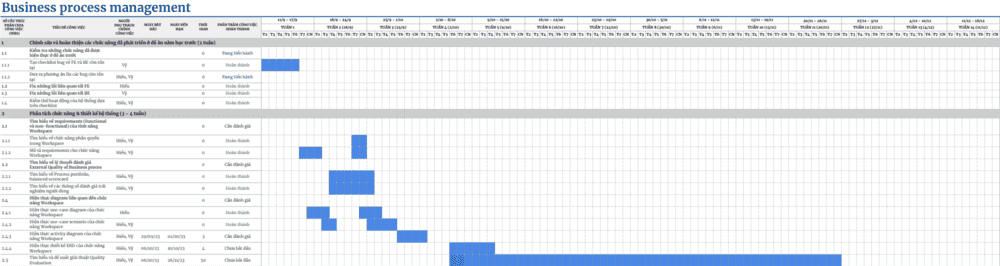
\includegraphics[width = \linewidth]{Content/Giới thiệu đề tài/images/PCCV_HK231_1.png}
    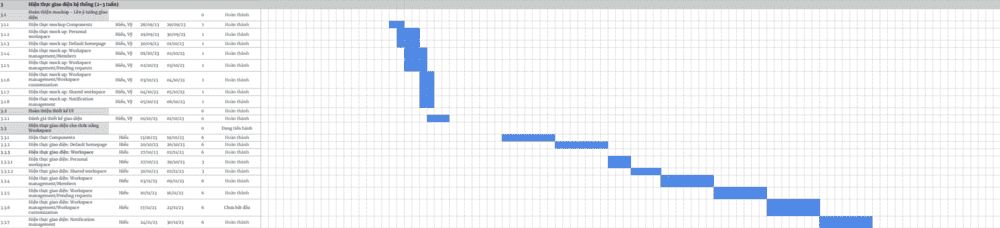
\includegraphics[width = \linewidth]{Content/Giới thiệu đề tài/images/PCCV_HK231_2.png}
    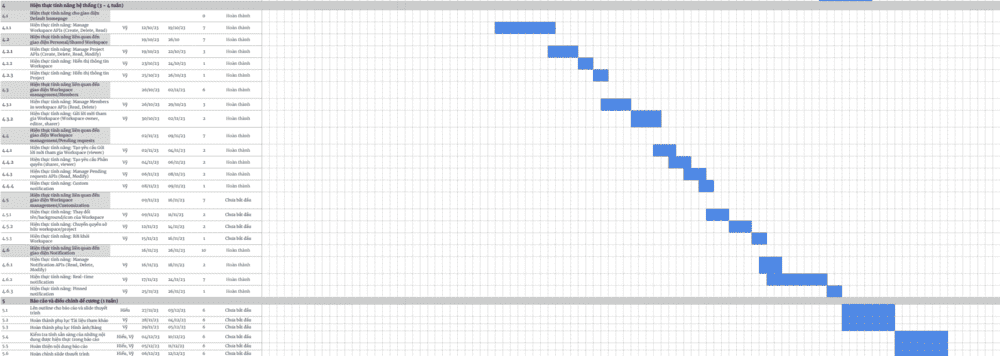
\includegraphics[width = \linewidth]{Content/Giới thiệu đề tài/images/PCCV_HK231_3.png}
    \vspace{0.5cm}
    \caption{Biểu đồ Gantt kế hoạch làm việc giai đoạn học kỳ HK231}
    \label{fig:Biểu đồ Gantt kế hoạch làm việc giai đoạn học kỳ HK231}
\end{figure}

\begin{table}[H]
    \centering
    \def\arraystretch{2}
    \resizebox{\textwidth}{!}{%
    \begin{tabular}{|p{11cm}|p{1.75cm}|p{1.5cm}|p{1.5cm}|}
    \hline
    Mô tả công việc & Phân công & Ngày bắt đầu & Ngày kết thúc 
    \\ \hline
    Hiện thực mockup Components                                             & Hiếu, Vỹ & 28/09/23 & 29/09/23 \\ \hline
    Hiện thực mock up: Personal workspace                                   & Hiếu, Vỹ & 29/09/23 & 30/09/23 \\ \hline
    Hiện thực mock up: Default homepage                                     & Hiếu, Vỹ & 30/09/23 & 01/10/23 \\ \hline
    Hiện thực mock up: Workspace management/Members                         & Hiếu, Vỹ & 01/10/23 & 02/10/23 \\ \hline
    Hiện thực mock up: Workspace management/Pending requests                & Hiếu, Vỹ & 02/10/23 & 03/10/23 \\ \hline
    Hiện thực mock up: Workspace management/Workspace customization         & Hiếu, Vỹ & 03/10/23 & 04/10/23 \\ \hline
    Hiện thực mock up: Shared workspace                                     & Hiếu, Vỹ & 04/10/23 & 05/10/23 \\ \hline
    Hiện thực mock up: Notification management                              & Hiếu, Vỹ & 05/10/23 & 06/10/23 \\ \hline
    Đánh giá thiết kế giao diện                                             & Hiếu, Vỹ & 01/10/23 & 01/10/23 \\ \hline
    Hiện thực Components                                                    & Hiếu     & 13/10/23 & 19/10/23 \\ \hline
    Hiện thực giao diện: Default homepage                                   & Hiếu     & 20/10/23 & 26/10/23 \\ \hline
    Hiện thực giao diện: Personal workspace                                 & Hiếu     & 27/10/23 & 29/10/23 \\ \hline
    Hiện thực giao diện: Shared workspace                                   & Hiếu     & 30/10/23 & 02/11/23 \\ \hline
    Hiện thực giao diện: Workspace management/Members                       & Hiếu     & 03/11/23 & 09/11/23 \\ \hline
    Hiện thực giao diện: Workspace management/Pending requests              & Hiếu     & 10/11/23 & 16/11/23 \\ \hline
    Hiện thực giao diện: Workspace management/Workspace customization       & Hiếu     & 17/11/23 & 23/11/23 \\ \hline
    Hiện thực giao diện: Notification management                            & Hiếu     & 24/11/23 & 30/11/23 \\ \hline
    Hiện thực tính năng: Manage Workspace APIs (Create, Delete, Read)       & Vỹ       & 12/10/23 & 19/10/23 \\ \hline
    Hiện thực tính năng: Manage Project APIs (Create, Delete, Read, Modify) & Vỹ       & 19/10/23 & 22/10/23 \\ \hline
    Hiện thực tính năng: Hiển thị thông tin Workspace                       & Vỹ       & 23/10/23 & 24/10/23 \\ \hline
    Hiện thực tính năng: Hiển thị thông tin Project                         & Vỹ       & 25/10/23 & 26/10/23 \\ \hline
    Hiện thực tính năng: Manage Members in workspace APIs (Read, Delete)    & Vỹ       & 26/10/23 & 29/10/23 \\ \hline
    Hiện thực tính năng: Gửi lời mời tham gia Workspace (Workspace owner, editor, sharer) & Vỹ       & 30/10/23 & 02/11/23 \\ \hline
    Hiện thực tính năng: Tạo yêu cầu Gửi lời mời tham gia Workspace (viewer)              & Vỹ       & 02/11/23 & 04/11/23 \\ \hline
    Hiện thực tính năng: Tạo yêu cầu Phân quyền (sharer, viewer)            & Vỹ       & 04/11/23 & 06/11/23 \\ \hline
    \end{tabular}%
    }
    \caption{Bảng kế hoạch công việc học kỳ HK231 - phần 1}
\end{table}

\begin{table}[H]
    \centering
    \def\arraystretch{2}
    \resizebox{\textwidth}{!}{%
    \begin{tabular}{|p{11cm}|p{1.75cm}|p{1.5cm}|p{1.5cm}|}
    \hline
    Hiện thực tính năng: Manage Pending requests APIs (Read, Modify)        & Vỹ       & 06/11/23 & 08/11/23 \\ \hline
    Hiện thực tính năng: Custom notification                                & Vỹ       & 08/11/23 & 09/11/23 \\ \hline
    Hiện thực tính năng: Thay đổi tên/background/icon của Workspace         & Vỹ       & 09/11/23 & 11/11/23 \\ \hline
    Hiện thực tính năng: Chuyển quyền sở hữu workspace/project              & Vỹ       & 12/11/23 & 14/11/23 \\ \hline
    Hiện thực tính năng: Rời khỏi Workspace                                 & Vỹ       & 15/11/23 & 16/11/23 \\ \hline
    Hiện thực tính năng: Manage Notification APIs (Read, Delete, Modify)    & Vỹ       & 16/11/23 & 18/11/23 \\ \hline
    Hiện thực tính năng: Real-time notification                             & Vỹ       & 17/11/23 & 24/11/23 \\ \hline
    Hiện thực tính năng: Pinned notification                                & Vỹ       & 25/11/23 & 26/11/23 \\ \hline
    Lên outline cho báo cáo và slide thuyết trình                           & Hiếu     & 27/11/23 & 03/12/23 \\ \hline
    Hoàn thành phụ lục Tài liệu tham khảo                                   & Vỹ       & 28/11/23 & 04/12/23 \\ \hline
    Hoàn thành phụ lục Hình ảnh/Bảng                                        & Vỹ       & 29/11/23 & 05/12/23 \\ \hline
    Kiểm tra tính sẵn sàng của những nội dung được hiện thực trong báo cáo                & Hiếu, Vỹ & 04/12/23 & 10/12/23 \\ \hline
    Hoàn thiện nội dung báo cáo                                             & Hiếu, Vỹ & 05/12/23 & 11/12/23 \\ \hline
    Hoàn chỉnh slide thuyết trình                                           & Hiếu, Vỹ & 06/12/23 & 12/12/23 \\ \hline
    \end{tabular}%
    }
    \caption{Bảng kế hoạch công việc học kỳ HK231 - phần 2}
\end{table}

\subsection{Giai đoạn học kỳ HK232}

\begin{figure} [H]
    \centering
    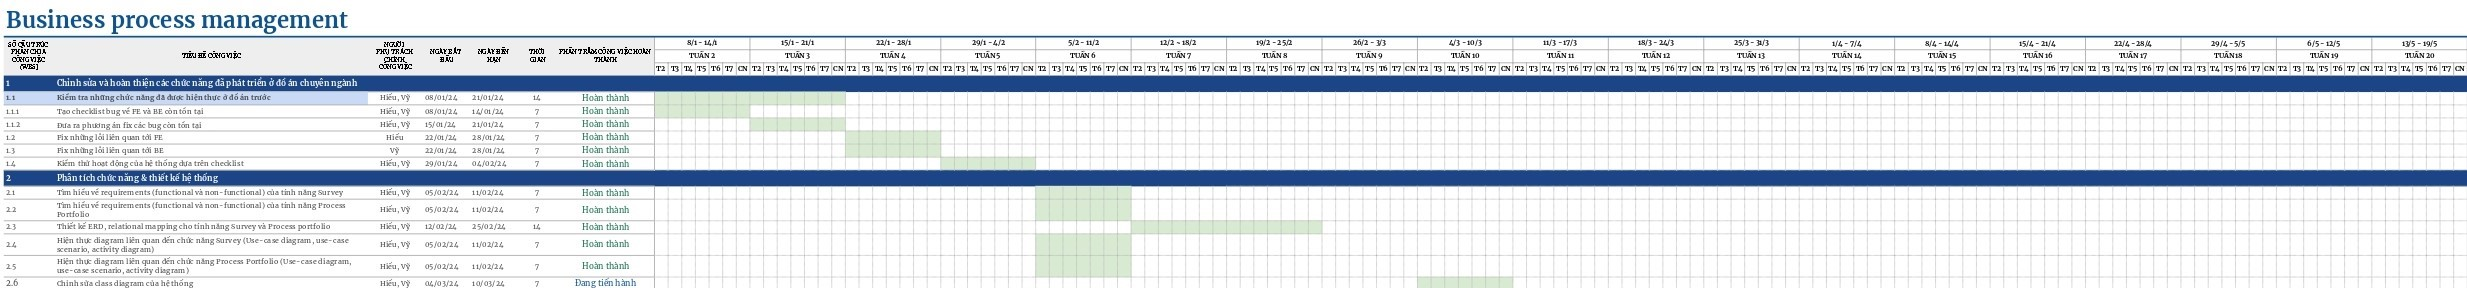
\includegraphics[width = \linewidth]{Content/Giới thiệu đề tài/images/PCCV_HK232_1.jpg}
    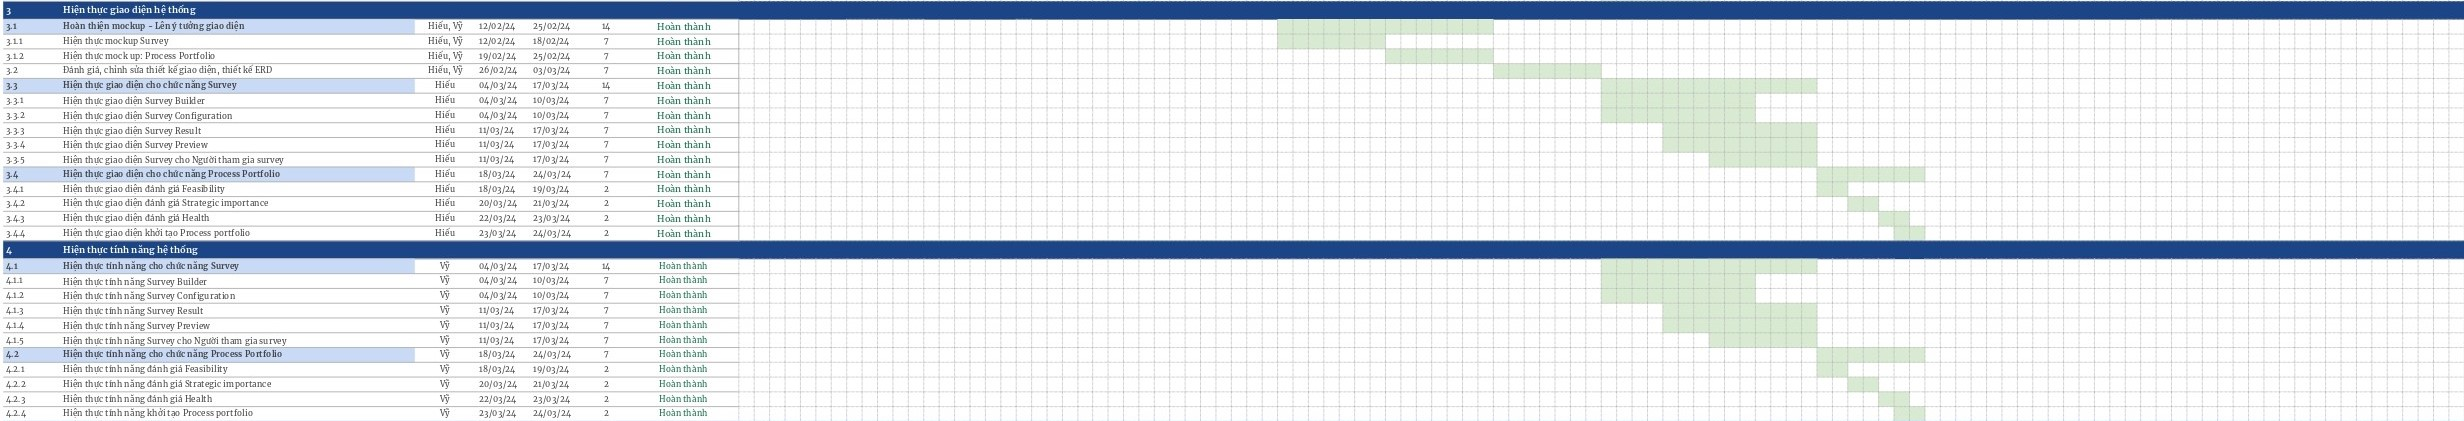
\includegraphics[width = \linewidth]{Content/Giới thiệu đề tài/images/PCCV_HK232_2.jpg}
    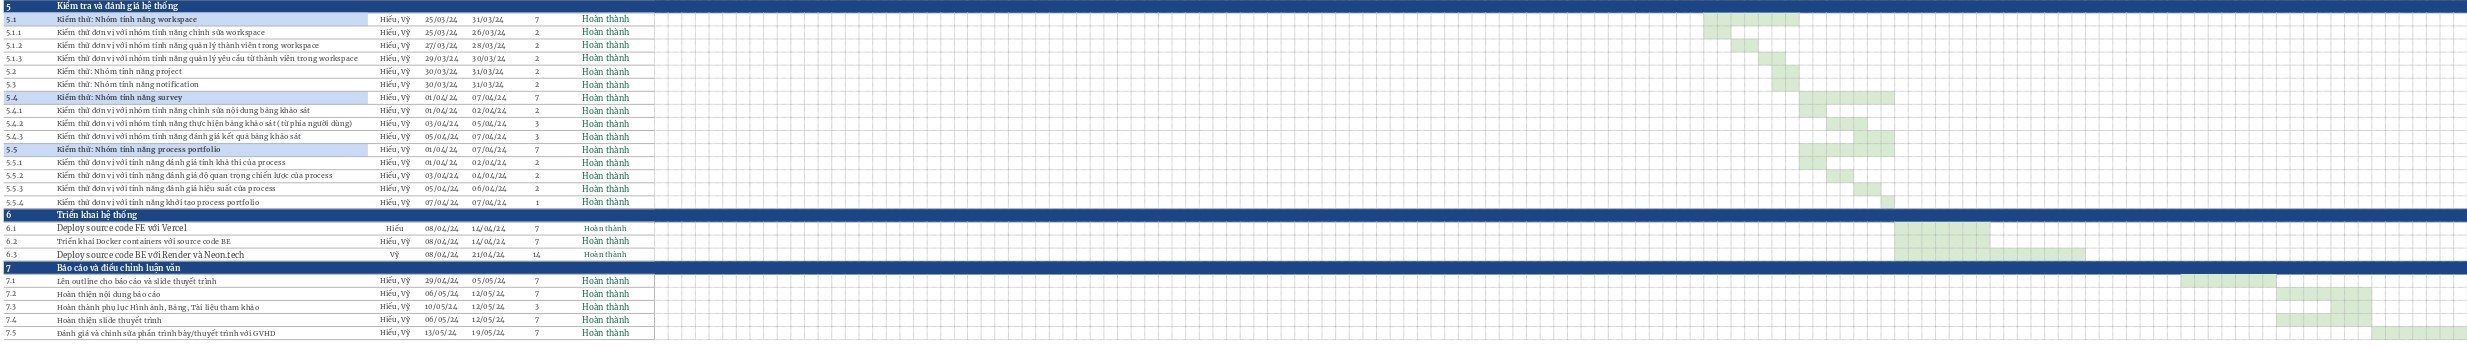
\includegraphics[width = \linewidth]{Content/Giới thiệu đề tài/images/PCCV_HK232_3.jpg}
    \vspace{0.5cm}
    \caption{Biểu đồ Gantt kế hoạch làm việc giai đoạn học kỳ HK232}
    \label{fig:Biểu đồ Gantt kế hoạch làm việc giai đoạn học kỳ HK232}
\end{figure}

\begin{table}[H]
    \centering
    \def\arraystretch{2}
    \resizebox{\textwidth}{!}{%
    \begin{tabular}{|p{11cm}|p{1.75cm}|p{1.5cm}|p{1.5cm}|}
    \hline
    Mô tả công việc & Phân công & Ngày bắt đầu & Ngày kết thúc
        \\ \hline
        {Tạo checklist bug về FE và BE còn tồn tại} &
        {Hiếu, Vỹ} &
        { 08/01/24} &
        { 14/01/24} \\ \hline
        { Đưa ra phương án fix các bug còn tồn tại} &
        { Hiếu, Vỹ} &
        { 15/01/24} &
        { 21/01/24} \\ \hline
        { Fix những lỗi liên quan tới FE} &
        { Hiếu} &
        { 22/01/24} &
        { 28/01/24} \\ \hline
        { Fix những lỗi liên quan tới BE} &
        { Vỹ} &
        { 22/01/24} &
        { 28/01/24} \\ \hline
        { Kiểm thử hoạt động của hệ thống dựa trên checklist} &
        { Hiếu, Vỹ} &
        { 29/01/24} &
        { 04/02/24} \\ \hline
        { Tìm hiểu về requirements (functional và non-functional) của tính năng Survey} &
        { Hiếu, Vỹ} &
        { 05/02/24} &
        { 11/02/24} \\ \hline
        { Tìm hiểu về requirements (functional và non-functional) của tính năng Process Portfolio} &
        { Hiếu, Vỹ} &
        { 05/02/24} &
        { 11/02/24} \\ \hline
        { Thiết kế ERD, relational mapping cho tính năng Survey và Process portfolio} &
        { Hiếu, Vỹ} &
        { 12/02/24} &
        { 25/02/24} \\ \hline
        { Hiện thực diagram liên quan đến chức năng Survey (Use-case diagram, use-case scenario, activity diagram)} &
        { Hiếu, Vỹ} &
        { 05/02/24} &
        { 11/02/24} \\ \hline
        { Hiện thực diagram liên quan đến chức năng Process Portfolio (Use-case diagram, use-case scenario, activity diagram)} &
        { Hiếu, Vỹ} &
        { 05/02/24} &
        { 11/02/24} \\ \hline
        { Chỉnh sửa class diagram của hệ thống} &
        { Hiếu, Vỹ} &
        { 04/03/24} &
        { 10/03/24} \\ \hline
        { Hiện thực mockup Survey} &
        { Hiếu, Vỹ} &
        { 12/02/24} &
        { 18/02/24} \\ \hline
        { Hiện thực mock up: Process Portfolio} &
        { Hiếu, Vỹ} &
        { 19/02/24} &
        { 25/02/24} \\ \hline
        { Đánh giá, chỉnh sửa thiết kế giao diện, thiết kế ERD} &
        { Hiếu, Vỹ} &
        { 26/02/24} &
        { 03/03/24} \\ \hline
        { Hiện thực giao diện Survey Builder} &
        { Hiếu} &
        { 04/03/24} &
        { 10/03/24} \\ \hline
        { Hiện thực giao diện Survey Configuration} &
        { Hiếu} &
        { 04/03/24} &
        { 10/03/24} \\ \hline
        { Hiện thực giao diện Survey Result} &
        { Hiếu} &
        { 11/03/24} &
        { 17/03/24} \\ \hline
        { Hiện thực giao diện Survey Result (trên toàn bộ câu hỏi)} &
        { Hiếu} &
        { 22/04/24} &
        { 28/04/24} \\ \hline{ Hiện thực giao diện Survey Preview} &
        { Hiếu} &
        { 11/03/24} &
        { 17/03/24} \\ \hline
        { Hiện thực giao diện Survey cho Người tham gia survey} &
        { Hiếu} &
        { 11/03/24} &
        { 17/03/24} \\ \hline
        { Hiện thực giao diện đánh giá Feasibility} &
        { Hiếu} &
        { 18/03/24} &
        { 19/03/24} \\ \hline
        { Hiện thực giao diện đánh giá Strategic importance} &
        { Hiếu} &
        { 20/03/24} &
        { 21/03/24} \\ \hline
        { Hiện thực giao diện đánh giá Health} &
        { Hiếu} &
        { 22/03/24} &
        { 23/03/24} \\ \hline
        { Hiện thực giao diện khởi tạo Process portfolio} &
        { Hiếu} &
        { 23/03/24} &
        { 24/03/24} \\ \hline
        { Hiện thực tính năng Survey Builder} &
        { Vỹ} &
        { 04/03/24} &
        { 10/03/24} \\ \hline
    \end{tabular}%
    }
    \caption{Bảng kế hoạch công việc học kỳ HK232 - phần 1}
\end{table}

\begin{table}[H]
    \centering
    \def\arraystretch{2}
    \resizebox{\textwidth}{!}{%
    \begin{tabular}{|p{11cm}|p{1.75cm}|p{1.5cm}|p{1.5cm}|}
    \hline
    Mô tả công việc & Phân công & Ngày bắt đầu & Ngày kết thúc
        \\ \hline
        { Hiện thực tính năng Survey Configuration} &
        { Vỹ} &
        { 04/03/24} &
        { 10/03/24} \\ \hline
        { Hiện thực tính năng Survey Result} &
        { Vỹ} &
        { 11/03/24} &
        { 17/03/24} \\ \hline
        { Hiện thức tính năng Survey Result (trên toàn bộ câu hỏi)} &
        { Vỹ} &
        { 22/04/24} &
        { 28/04/24} \\ \hline
        { Hiện thực tính năng Survey Preview} &
        { Vỹ} &
        { 11/03/24} &
        { 17/03/24} \\ \hline
        { Hiện thực tính năng Survey cho Người tham gia survey} &
        { Vỹ} &
        { 11/03/24} &
        { 17/03/24} \\ \hline
        { Hiện thực tính năng đánh giá Feasibility} &
        { Vỹ} &
        { 18/03/24} &
        { 19/03/24} \\ \hline
        { Hiện thực tính năng đánh giá Strategic importance} &
        { Vỹ} &
        { 20/03/24} &
        { 21/03/24} \\ \hline
        { Hiện thực tính năng đánh giá Health} &
        { Vỹ} &
        { 22/03/24} &
        { 23/03/24} \\ \hline
        { Hiện thực tính năng khởi tạo Process portfolio} &
        { Vỹ} &
        { 23/03/24} &
        { 24/03/24} \\ \hline
        { Kiểm thử đơn vị với nhóm tính năng chỉnh sửa workspace} &
        { Hiếu, Vỹ} &
        { 25/03/24} &
        { 26/03/24} \\ \hline
        { Kiểm thử đơn vị với nhóm tính năng quản lý thành viên trong workspace} &
        { Hiếu, Vỹ} &
        { 27/03/24} &
        { 28/03/24} \\ \hline
        { Kiểm thử đơn vị với nhóm tính năng quản lý yêu cầu từ thành viên trong workspace} &
        { Hiếu, Vỹ} &
        { 29/03/24} &
        { 30/03/24} \\ \hline
        { Kiểm thử: Nhóm tính năng project} &
        { Hiếu, Vỹ} &
        { 30/03/24} &
        { 31/03/24} \\ \hline
        { Kiểm thử: Nhóm tính năng notification} &
        { Hiếu, Vỹ} &
        { 30/03/24} &
        { 31/03/24} \\ \hline
        { Kiểm thử đơn vị với nhóm tính năng chỉnh sửa nội dung bảng khảo sát} &
        { Hiếu, Vỹ} &
        { 01/04/24} &
        { 02/04/24} \\ \hline
        { Kiểm thử đơn vị với nhóm tính năng thực hiện bảng khảo sát (từ phía người dùng)} &
        { Hiếu, Vỹ} &
        { 03/04/24} &
        { 05/04/24} \\ \hline
        { Kiểm thử đơn vị với nhóm tính năng đánh giá kết quả bảng khảo sát} &
        { Hiếu, Vỹ} &
        { 05/04/24} &
        { 07/04/24} \\ \hline
        { Kiểm thử đơn vị với tính năng đánh giá tính khả thi của process} &
        { Hiếu, Vỹ} &
        { 01/04/24} &
        { 02/04/24} \\ \hline
        { Kiểm thử đơn vị với tính năng đánh giá độ quan trọng chiến lược của process} &
        { Hiếu, Vỹ} &
        { 03/04/24} &
        { 04/04/24} \\ \hline
        { Kiểm thử đơn vị với tính năng đánh giá hiệu suất của process} &
        { Hiếu, Vỹ} &
        { 05/04/24} &
        { 06/04/24} \\ \hline
        { Kiểm thử đơn vị với tính năng khởi tạo process portfolio} &
        { Hiếu, Vỹ} &
        { 07/04/24} &
        { 07/04/24} \\ \hline
        { Deploy source code FE với Vercel} &
        { Hiếu} &
        { 08/04/24} &
        { 14/04/24} \\ \hline
        { Triển khai Docker containers với source code BE} &
        { Hiếu, Vỹ} &
        { 08/04/24} &
        { 14/04/24} \\ \hline
        { Deploy source code BE với Render và Neon.tech} &
        { Vỹ} &
        { 08/04/24} &
        { 21/04/24} \\ \hline
        { Lên outline cho báo cáo và slide thuyết trình} &
        { Hiếu, Vỹ} &
        { 29/04/24} &
        { 05/05/24} \\ \hline
        { Hoàn thiện nội dung báo cáo} &
        { Hiếu, Vỹ} &
        { 06/05/24} &
        { 12/05/24} \\ \hline 
    \end{tabular}%
    }
    \caption{Bảng kế hoạch công việc học kỳ HK232 - phần 2}
\end{table}

\begin{table}[H]
    \centering
    \def\arraystretch{2}
    \resizebox{\textwidth}{!}{%
    \begin{tabular}{|p{11cm}|p{1.75cm}|p{1.5cm}|p{1.5cm}|}
    \hline
    Mô tả công việc & Phân công & Ngày bắt đầu & Ngày kết thúc
        \\ \hline
        { Hoàn thành phụ lục Hình ảnh, Bảng, Tài liệu tham khảo} &
        { Hiếu, Vỹ} &
        { 10/05/24} &
        { 12/05/24} \\ \hline
        { Hoàn thiện slide thuyết trình} &
        { Hiếu, Vỹ} &
        { 06/05/24} &
        { 12/05/24} \\ \hline
        { Đánh giá và chỉnh sửa phần trình bày/thuyết trình với GVHD} &
        { Hiếu, Vỹ} &
        { 13/05/24} &
        { 19/05/24} \\ \hline
    \end{tabular}%
    }
    \caption{Bảng kế hoạch công việc học kỳ HK232 - phần 3}
\end{table}